%%%%%%%%%%%%%%%%%%%%%%%%%%%%%%%%%%%%%%%%%%%%%%%%%%%%%%%%%%%%%%%%%%%%%%%%%%%%%%%%
%2345678901234567890123456789012345678901234567890123456789012345678901234567890
%        1         2         3         4         5         6         7         8

%\documentclass[letterpaper, 10 pt, conference]{ieeeconf}  % Comment this line out if you need a4paper

\documentclass[a4paper, 10pt, conference]{ieeeconf}      % Use this line for a4 paper

\IEEEoverridecommandlockouts                              % This command is only needed if 
                                                          % you want to use the \thanks command

\overrideIEEEmargins                                      % Needed to meet printer requirements.

% See the \addtolength command later in the file to balance the column lengths
% on the last page of the document

% The following packages can be found on http:\\www.ctan.org
%\usepackage{graphics} % for pdf, bitmapped graphics files
%\usepackage{epsfig} % for postscript graphics files
%\usepackage{mathptmx} % assumes new font selection scheme installed
%\usepackage{times} % assumes new font selection scheme installed
%\usepackage{amsmath} % assumes amsmath package installed
%\usepackage{amssymb}  % assumes amsmath package installed
\usepackage{amssymb,url,amsmath}
\usepackage{algorithm}
\usepackage{graphicx}
\usepackage{epstopdf}
\usepackage{textcomp}
\usepackage{color}
\usepackage{ifpdf}
\usepackage{url}
\usepackage{enumerate}
\usepackage{array}
\usepackage{flushend}
\usepackage{multirow,booktabs}
\usepackage{hyperref}
\usepackage{subfig}
\usepackage{mdwlist}
\usepackage[utf8]{inputenc}
\usepackage{tcolorbox}
\newcommand{\alg}{Algorithm~}
\newtcolorbox[auto counter]{algorithmbox}[2][]{colback=red!5!white,colframe=red!75!black,fonttitle=\bfseries, title=\alg\thetcbcounter: #2,#1}

\newcommand{\eq}{Eq.~}
\newcommand{\fig}{Fig.~}
\newcommand{\tab}{Tab.~}
\newcommand{\sect}{Sec.~}

\newcommand{\re}{R}
\newcommand{\rf}{R}
\newcommand{\rl}{L}
\newcommand{\om}{O}
\newcommand{\cm}{M}
\newcommand{\fm}{F}
\newcommand{\hc}{C}
\newcommand{\qd}{Q}
\newcommand{\gpm}{T}
\newcommand{\coll}{W}
\newcommand{\pdf}{\mathbf{pdf}}

\newcommand{\argmax}[1]{\underset{#1}{\operatorname{argmax}}\medspace}

\title{\LARGE \bf
Learning and Inference of Dexterous Grasps for Novel Objects with Underactuated Hands
}

\author{Marek Kopicki$^{1}$ and Carlos J. Rosales$^{2}$ and Hamal Marino$^{2}$ and Marco Gabiccini$^{2}$ and Jeremy L. Wyatt$^{1}$% <-this % stops a space
\thanks{*This work was supported by EC-FP7-ICT-600918, PacMan.}% <-this % stops a space
\thanks{$^{1}$Marek Kopicki and Jeremy L. Wyatt are with the Intelligent Robotics Laboratory, School of Computer Science,
        University of Birmingham, Birmingham, B15 2TT, UK.
        {\tt\small \{msk,jlw\}@cs.bham.ac.uk}}%
\thanks{$^{2}$Carlos Rosales, Hamal Marino and Marco Gabiccini are with Centro Piaggio, Universita di Pisa, Pisa, Italy.
               {\tt\small carlos.rosales@for.unipi.it, hamal.marino@centropiaggio.unipi.it, m.gabiccini@ing.unipi.it}}%
}
\begin{document}


\maketitle
\thispagestyle{empty}
\pagestyle{empty}


%%%%%%%%%%%%%%%%%%%%%%%%%%%%%%%%%%%%%%%%%%%%%%%%%%%%%%%%%%%%%%%%%%%%%%%%%%%%%%%%
\begin{abstract}
Recently, advances have been made in learning of grasps for fully actuated hands. A typical approach is to learn the target locations of finger links on the object surface. When a new object must be grasped, new finger locations are generated, and a collision free reach-to-grasp trajectory is planned. Such a division of labour fails to exploit the advantages of underactuated hands, which improve grasp reliability via contacts with the object during grasping. In this paper we present a method for learning grasps for underactuated hands. Our approach works by learning not only the desired final grasp, but also good grasping trajectories. We learn these trajectories from example grasps generated with a rigid body simulation of hand and object. This enables us to learn how to approach the object and close the underactuated hand so as to induce a favourable sequence of contacts. Our method does not rely on explicit representation of the contact sequence. The core learning method uses a product of experts approach. This allows grasp transfer to novel objects and works despite partial shape reconstruction.


\end{abstract}


%%%%%%%%%%%%%%%%%%%%%%%%%%%%%%%%%%%%%%%%%%%%%%%%%%%%%%%%%%%%%%%%%%%%%%%%%%%%%%%%
\section{INTRODUCTION}

Transferring dexterous grasps to novel objects is a challenging problem. One approach is to machine learn solutions with techniques able to perform powerful generalisation. Another is to use an underactuated hand to cope with shape variation. In this paper we combine the benefits of both approaches by learning grasps for underactuated hands. Underactuated hands exploit the contacts that occur during grasping to achieve a wide variety of final grasp configurations. The final grasp configuration depends not only on the final hand pose, but also on the object shape, and on the reach to grasp trajectory. An interesting challenge is to use machine learning to exploit these interactions. The key technical challenge in applying machine learning to grasping with underactuated hands is to learn the right trajectory for a particular object shape so as to achieve a good grasp of a particular type. 

One approach would be to learn the typical contact interactions that occur during a grasp, and to generate new grasps that reproduce these. The contact interactions are, however, rather complex and variable, even given small variations in object shape and friction. Therefore we tackle the problem by implicitly encoding the contact interactions in terms of the approach trajectory. Our method learns both the desired final contacts, the final hand shape, and the hand pose during the reach to grasp trajectory. We build on our previous work on one-shot learning of grasps that transfer to novel objects, employing a product of experts formulation. The method is able to learn a flexible grasp from examples generated in physics simulation. It copes with partial and noisy shape information for the test objects. The method requires no knowledge of the human defined object category, either when learning or performing transfer.

\section{RELATED WORK}
Previous work in learning generalisable grasps falls broadly into two classes. One class of approaches utilises the shape of common object parts or their appearance to generalise grasps across object categories \cite{saxena2008b,detry2013a,herzog2014a, kroemer2012a}. This works well for low DoF hands. Another class of approaches captures the global properties of the hand shape either at the point of grasping, or during the approach \cite{ben2012generalization}. This global hand shape can additionally be associated with global object shape, allowing generalisation by warping grasps to match warps of global object shape \cite{hillenbrand2012transferring}. This second class works well for high DoF hands, but generalisation is more limited. We have previously achieved the advantages of both classes, generalising grasps across object categories with high DoF hands. In this paper we go beyond this, learning and generalising grasps for under-actuated hands.

We now sketch the representations underpinning our approach. We define several models: an object model (partial and acquired from sensing); a model of the contact between a finger link and the object; a model of the whole hand configuration; and a model of the reach to grasp trajectory. First we describe the kernel density representation for all these models. Then we describe the surface features we use to encode some of these models. We assume that the robot's hand comprises $N_L$ rigid \emph{links}: a palm, and several phalanges or links. We denote the set of links $L =\{L_i\}$.

\subsection{Kernel Density Estimation}
\label{sec:kde}
$SO(3)$ denotes the group of rotations in three dimensions. A feature belongs to the space $SE(3) \times \mathbb R^2$, where $SE(3) = \mathbb R^3 \times SO(3)$ is the group of 3D \emph{poses}, and surface descriptors are composed of two real numbers. We extensively use probability density functions (PDFs) defined on $SE(3) \times \mathbb R^2$.  We represent these PDFs non-parametrically with a set of $K$ features (or particles) $x_j$
\begin{equation}
S = \left\lbrace x_j : x_j \in \mathbb R^3 \times SO(3) \times \mathbb R^2 \right\rbrace_{j \in [1,K]}.
\end{equation}
The probability density in a region is determined by the local density of the particles in that region. The underlying PDF is created through \emph{kernel density estimation} \cite{silverman1986a}, by assigning a kernel function $\mathcal{K}$ to each particle supporting the density, as
\begin{equation}\label{eq:d}
\pdf(x) \simeq \sum_{j=1}^K w_j \mathcal{K}(x| x_{j}, \sigma),
\end{equation}
where  $\sigma \in \mathbb R^3$ is the kernel bandwidth and $w_j \in \mathbb R^{+}$ is a weight associated to $x_j$ such that $\sum_j w_j = 1$. We use a kernel that factorises into three functions defined by the separation of $x$ into $p \in \mathbb R^3$ for position, a quaternion $q \in SO(3)$ for orientation, and $r \in \mathbb R^2$ for the surface descriptor. Furthermore, let us denote by $\mu$ another feature, and its separation into position, orientation and a surface descriptor. Finally, we denote by $\sigma$ a triplet of real numbers:
\begin{subequations}
\begin{align}
x &= (p, q, r),\\
\mu &= (\mu_p, \mu_q, \mu_r),\\
\sigma &= (\sigma_p, \sigma_q, \sigma_r).
\end{align}
\label{eq:feature}
\end{subequations}
We define our kernel as
\begin{equation}\label{eq:kernel_in_se3}
\mathcal{K}(x| \mu, \sigma) = \mathcal{N}_3(p| \mu_p, \sigma_p) \Theta(q| \mu_q, \sigma_q) \mathcal{N}_2(r| \mu_r, \sigma_r)
\end{equation}
where $\mu$ is the kernel mean point, $\sigma$ is the kernel bandwidth, $\mathcal{N}_n$ is an $n$-variate isotropic Gaussian kernel, and ${\Theta}$ corresponds to a pair of antipodal von Mises-Fisher distributions which form a Gaussian-like distribution on $SO(3)$ \cite{fisher1953a,sudderth2006a}. The value of ${\Theta}$ is given by
\begin{equation}
\Theta(q|\mu_q, \sigma_q) = C_4(\sigma_q) \frac {e^{\sigma_q \; \mu_q^T q} + e^{-\sigma_q \; \mu_q^T q}}2
\end{equation}
where $C_4(\sigma_q)$ is a normalising constant, and $\mu_q^T q$ denotes the quaternion dot product.

Using this representation, conditional and marginal probabilities can easily be computed from \eq\eqref{eq:d}. The marginal density $\pdf(r)$ is computed as
\begin{align}\label{eq:marginal}
\pdf(r) & \\
      = & \iint \sum_{j=1}^K w_j \mathcal{N}_3(p| p_i, \sigma_p) \Theta(q| q_i, \sigma_q) \mathcal{N}_2(r| r_i, \sigma_r) \textnormal{d}p\textnormal{d}q \\
      = &  \sum_{j=1}^K w_j \mathcal{N}_2(r| r_j, \sigma_r),
\end{align}
where $x_j = (p_j, q_j, r_j)$.
The  conditional density $\pdf(p,q|r)$ is given by
\begin{align}\label{eq:conditional}
\pdf(p,q|{r}) & = \frac{\pdf(p, q, {r})}{\pdf({r})} \\
                   & = \frac{\sum_{j=1}^K w_j \mathcal{N}_2({r}| r_j, \sigma_r) \mathcal{N}_3(p| p_j, \sigma_p) \Theta(q|q_j, \sigma_q)}{\sum_{j=1}^K w_j \mathcal{N}_2({r}| r_j, \sigma_r)}. 
\end{align}

\subsection{Surface Features}
\label{sec:surface_features}

All objects considered in the paper are represented by point clouds constructed from one or multiple shots taken by a depth camera. We directly augment these points with a frame of reference and a surface feature that is a local curvature descriptor. For compactness, we also denote the pose of a feature as $v$. As a result,
\begin{equation}
x = (v, r), \qquad v = (p, q).
\label{eq:surface.feature}
\end{equation}

The surface normal at $p$ is computed from the nearest neighbours of $p$ using a PCA-based method (e.g. \cite{kanatani2005statistical}). The surface descriptors are the local \emph{principal curvatures} \cite{spivak1979comprehensive}. Their directions are denoted $k_1, k_2 \in \mathbb R^3$, and the curvatures along $k_1$ and $k_2$ form a $2$-dimensional feature vector $r = (r_1, r_2) \in \mathbb R^2$. %The surface normals and curvatures are computed using the PCL library \citep{Rusu_ICRA2011_PCL}.
The surface normal and the principal directions define the orientation $q$ of a frame that is associated with the point $p$. 

Thus, given a point cloud, a set of $K_O$ features  $\lbrace (v_j, r_j) \rbrace$ can be computed. This set of features defines, in turn, a joint probability distribution, which we call the \emph{object model}:
\begin{equation}
\om(v, r) \equiv \pdf^\om(v, r) \simeq \sum_{j=1}^{K_O} w_j \mathcal{K}(v, r|{x_j}, \sigma_{x})
%RD: mu and sigma are not properly defined.
\label{eq:om}
\end{equation}
where $\om$ is short for $\pdf^\om$, $x_j = (v_j, r_j)$,  $\mathcal{K}$ is defined in \eq\eqref{eq:kernel_in_se3} with bandwidth $\sigma_{x} = (\sigma_{v}, \sigma_{r})$, and where all weights are equal, $w_j = 1/{K_O}$. We refer to $\om$ as the object model. In summary this object model represents the object as a pdf over surface normals and curvatures.

\subsection{Contact Model}\label{sec:contact.model}

A contact model $\cm_i$ encodes the joint probability distribution of surface curvatures and of the 3D pose of the $i$-th hand link. Intuitively Let us consider the hand grasping some given object. The (object) contact model of link $\rl_i$ is denoted by
\begin{equation}\label{eq:M}
\cm_i(U, R) \equiv \pdf^\cm_i(U, R)
\end{equation}
where $\cm_i$ is short for $\pdf^\cm_i$, $R$ is the random variable modelling surface curvature, and $U$ models the pose of $\rl_i$ \emph{relative} to the frame of reference defined by the directions of principal curvature. In other words, denoting realisations of $R$ and $U$ by $r$ and $u$, $\cm_i(u, r)$ is proportional to the probability of finding $\rl_i$ at pose $u$ relative to the frame of a nearby object surface patch that exhibits principal curvatures equal to $r$.

Given a set of features $\lbrace x_j \rbrace_{j=1}^{K_O}$, with $x_j = (v_j, r_j)$ and $v_j = (p_j, q_j)$, a contact model $\cm_i$ is constructed from them.  Features close to the link surface are more important than those lying far from the surface. Features are thus weighted, to make their influence on $\cm_i$  decrease with their distance to the $i^\textnormal{th}$ link (\fig\ref{fig:representations.modeldist.cont}). We use a weighting function whose value decreases exponentially with the square distance to the link:
\begin{equation}
w_{ij} = \begin{cases}\exp(-\lambda ||p_j-a_{ij}||^2) \quad &\textnormal{ if } ||p_j-a_{ij}|| < \delta_i\\
0 \quad &\textnormal{ otherwise},\end{cases}
\label{eq:learning.modeldist.wgh}
\end{equation}
where $\lambda \in \mathbb R^{+}$ and $a_{ij}$ is the point on the surface of $\rl_i$ that is closest to $p_j$. The intuitive motivation for this choice is that we require a weight function that falls off quickly so that the contact model will only take account of the local shape, while falling off smoothly.

Let us denote by $u_{ij} = (p_{ij}, q_{ij})$ the pose of $\rl_i$ relative to the pose $v_j$ of the $j^{\mathnormal{th}}$ surface feature. In other words, $u_{ij}$ is defined as
\begin{equation}
u_{ij} = v_j^{-1} \circ s_i,
\label{eq:local.pose}
\end{equation}
where $s_i$ denotes the pose of $\rl_i$, $\circ$ denotes the pose composition operator, and $v_j^{-1}$ is the inverse of $v_j$, with $v_j^{-1} = (-q_j^{-1}p_j, q_j^{-1})$ (see \fig\ref{fig:representations.model}). The contact model is estimated as
\begin{equation}
\cm_i(u,r) \simeq \frac 1Z \sum^{K_{M_i}}_{j=1} w_{ij}\mathcal{N}_3(p|{p_{ij}}, \sigma_{p}) \Theta(q|{q_{ij}}, \sigma_{q}) \mathcal{N}_2(r|{r_j}, \sigma_{r})
\label{eq:cm}
\end{equation}
where $Z$ is a normalising constant, $u = (p, q)$, and where $K_{M_i} \leq K_O$ is a number of features which are within cut-off distance $\delta_i$ to the surface of link $\rl_i$. If the number of features $K_{M_i}$ of contact model $\cm_i$ is not sufficiently large, contact model $\cm_i$ is not instantiated and is excluded from any further computation. Consequently, the overall number of contact models $N_M$ is usually smaller than the number of links $N_L$ of the robotic hand. We denote the set of contact models learned from a grasp example $g$ as $\mathcal{M}^g=\{\mathcal{M}^g_i\}$. The contact models are quite different for the different links within a grasp. This can be seen by comparing the marginalised contact models $\cm(r)$ for two example training grasps and two links in \fig\ref{fig:representations.features}.

%Sum~\eqref{eq:cm} involves only terms for which $x_j = ((p_j, q_j), r_j)$ belong to the neighbourhood of $\rf_i$, $\lbrace x_j: ||p_j-a_{ij}|| \leq \delta, \delta \in \mathbb R^{+} \rbrace$. If the neighbourhood of a particular link $i$ is empty, i.e. $K_{M_i} = 0$, the corresponding contact model is not instantiated and it is excluded from any further computation.
\begin{figure}[t]
\centerline{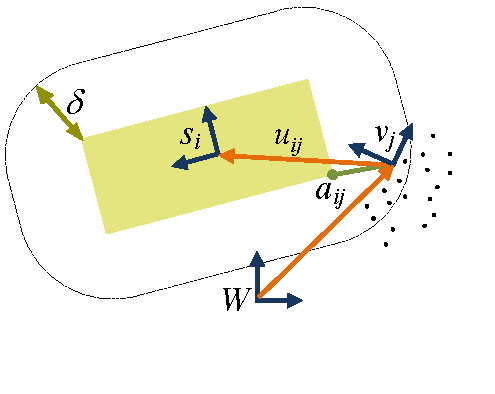
\includegraphics[width=5cm]{resources/model}}
\caption[Contact model]{Contact model. The figure shows the $i$-th link $\rl_i$ (solid block) and its pose $s_i$. The black dots are samples of the surface of an object. The distance $a_{ij}$ between a feature $v_j$ and the closest point on the link's surface is shown. The rounded rectangle illustrates the cut-off distance $\delta_i$. The poses $v_j$ and $s_i$ are expressed in the world frame $W$. The arrow $u_{ij}$ is the pose of $\rl_i$ relative to the frame for the surface feature $v_j$.}
\label{fig:representations.model}
\end{figure}

The parameters $\lambda$ and $\sigma_{p}$, $\sigma_{q}$, $\sigma_{r}$ were chosen empirically and kept fixed in all experiments reported in \sect\ref{sec:method}. The time complexity for learning each contact model from an example grasp is $\Omega(T K_O)$ where $T$ is the number of triangles in the tri-mesh describing the hand links, and $K_O$ is the number of points in the object model.


%\begin{figure}[t]
%\centering{
%\subfloat[]{\includegraphics[height=3.4cm]{resources/example1}}\quad
%\subfloat[]{\includegraphics[height=3.4cm]{resources/example2}}\quad
%\subfloat[]{\includegraphics[height=3.4cm]{resources/example5}}
%}
%\caption[Hand-object contact]{Example top grasp of a mug represented by a point cloud (panel a). The dotted regions are rays between features and the closest hand link surfaces (panel b). The black curves with frames at the fingertips represent the range of hand configurations in \eq\eqref{eq:hc} (panel c).}
%\label{fig:representations.modeldist.cont}
%\end{figure}

\subsection{Hand Configuration Model}

The hand configuration model, denoted by $\hc$, encodes a set of configurations of the hand joints $h_c \in \mathbb R^D$ (i.e., joint angles), that are particular to a grasp example. The purpose of this model is to allow us to restrict the grasp search space (during grasp transfer) to hand configurations that resemble those observed while training the grasp.

In order to boost the generalisation capability of the grasping algorithm the hand configuration model encodes the hand configuration that was observed when grasping the training object, but also a set of configurations recorded during the approach towards the object. Let us denote by $h^t_c$ the joint angles at some small distance \emph{before} the hand reached the training object, and by $h^g_c$ the hand joint angles at the time when the hand made contact with the training object. We consider a set of configurations interpolated between $h^t_c$ and $h^g_c$, and extrapolated beyond $h^g_c$, as
\begin{equation}
h_c(\gamma) = (1 - \gamma)h^g_c + \gamma h^t_c
\label{eq:learning.configmodel.config}
\end{equation}
\noindent where $\gamma \in \mathbb R$. For all $\gamma < 0$, configurations $h_c(\gamma)$ are beyond $h^g_c$ (see \fig\ref{fig:representations.modeldist.cont}). The hand configuration model $\hc$ is constructed by applying kernel density estimation to \begin{equation}\label{eq:H_c}\mathcal H_c = \lbrace h_c(\gamma): \gamma \in [-\beta, \beta], \beta \in \mathbb R^{+}\rbrace,\end{equation} as 
\begin{equation}
\hc(h_c) \equiv \sum_{\gamma \in [-\beta, \beta]} w({h_c(\gamma)}) \mathcal{N}_D(h_c|h_c(\gamma), \sigma_{h_c}) 
\label{eq:hc}
\end{equation}
where  $w({h_c(\gamma)}) = \exp(-\alpha \|h_c(\gamma) - h^g_c \|^2)$ and $\alpha \in \mathbb R^{+}$. $\alpha$ and $\beta$ were hand tuned and kept fixed in all the experiments. The hand configuration model computation has time complexity $\Omega(d_h K_C)$ where $d_h$ is the number of dimensions of the configuration vector, and $K_C$ is the size of the set of values of $\gamma$ used in \eq\eqref{eq:hc}.

\subsection{Reach to Grasp Trajectory}

We encode a reach to grasp trajectory as the combined trajectory of the wrist pose and the hand configuration. Each wrist pose is defined in the frame of reference of the final wrist pose in the trajectory. This final wrist pose is associated with the final hand configuration model and the contact models. We refer to the final hand configuration model, wrist pose and contact models as the model of the final grasp state.  A set of reach to grasp trajectories, including the final grasp states can be defined. We create this set so that the final grasp states are all very close to one another, thus forming an attractor, with the trajectories leading to those similar final grasp states defining an attractor basin.


\section{LEARNING}

SAY HOW WE USE THE SIMULATOR HERE

\section{INFERENCE}

NEED TO ADAPT FOR SOFT HAND (TRAJECTORY + CONTACT MODEL)

\section{Inferring Grasps for Novel Objects}
\label{sec:infer}

After acquiring the contact model and the configuration model, the robot is now presented with a new query object to grasp. The aim is that the robot finds a generalisation of a training grasp such that its links are well-placed with respect to the object surface, while preserving similarity to the example grasp. We infer generalised grasps for every example grasp, and pick the transfer grasp that is most likely according to the learned models.

%First of all the contact models are combined with the observed point cloud for the object to obtain a set of \emph{query densities}, one for each hand part. Query density $\qd_i$ is a density over 3D poses of the $i$-th hand part $\rl_i$ in the world coordinates. A grasping hand pose is found by simultaneously maximising query densities $\qd_i$ of all (involved) hand parts together with an additional constraint provided by the hand configuration model $\hc$ in a single optimisation procedure. The hand configuration model limits possible hand joint configurations to a (sub)space of hand postures specific to the example grasps. Each joint configuration together with the hand forward kinematics determines the mutual spatial locations between the hand parts, leaving only one additional free parameter ($\mathbb R^3 \times SO(3)$ vector) to optimise - the hand wrist pose in world coordinates.

First of all we combine each of the contact models with the query object's perceived point cloud, to obtain a set of {\em query densities}, one for each link that has an associated contact model. The $i$-th query density $\qd_i$ is a density modelling where the $i$-th link can be placed, with respect to the surface of a new object (see \fig\ref{fig:grasping.querydensity}). From the query densities, a hand pose is generated as follows. We randomly pick a link $i$. We randomly sample, from the corresponding query density $\qd_i$, a pose for link $i$. We sample, from the configuration model $\hc$, a hand configuration that is compatible with the pose selected for link $i$, and then we compute from forward kinematics the 3D poses of all the remaining hand links. We refine the grasp by performing a simulated annealing search in the hand configuration space, to locally maximise the grasp likelihood measured as the product of the hand configuration density and the query densities for all the hand links.
%, to make contacts with surface patches of similar local curvature to their contact models. % this last sentence disturbs me..
We repeat the entire process a number of times, and select the most likely grasp that is also kinematically feasible.

%In summary our algorithm generates many possible grasps, each with its likelihood. Each grasp has a set of hand part poses that independently comply with the contact models, while jointly complying to the hand configuration model. We now explain in detail how we create a pdf so that we can sample poses for a single hand part, given the observation of a novel object. The section following it explains the simulated annealing process for refining the whole grasp.

The optimisation procedure generates many possible grasps, each with its likelihood. Each grasp has a set of link poses that independently comply with the contact models, while jointly complying with the hand configuration model.

This section explains how query densities are constructed. A query density results from the combination of a contact model for a specific finger link with an object point cloud $\om$ for the new object. The purpose of a query density is both to generate and evaluate poses of the corresponding finger link on the new object. The $i$-th query density $\qd_i$ models the pose $s$ {\em in the world frame} of the $i$-th link $\rl_i$.

A query density should be defined in a way that achieves good generalisation from training to test objects. We define our query density \eqref{eq:qd} by $K_{Q_i}$ kernels centred on the set of weighted finger link poses returned by \alg\ref{alg:mc}:
\begin{equation}
\qd_i(s) \simeq \sum^{K_{Q_i}}_{j=1} w_{ij} \mathcal{N}_3(p|{\hat{p}_{ij}}, \sigma_{p}) \Theta(q|{\hat{q}_{ij}}, \sigma_{q})%, \quad i = 1, ..., N_L
\label{eq:qd.approx}
\end{equation}
with $j$-th kernel centre $({\hat{p}_{ij}}, {\hat{q}_{ij}}) = \hat{s}_{ij}$, and where all weights were normalised $\sum_j w_{ij} = 1$. The number of kernels $K_{Q_i} = K_Q$ were chosen equal for all query densities and grasp types (unless otherwise stated). The non-Euclidean domain on which our density estimates are computed makes it difficult and computationally expensive to find optimal values for the bandwidth $\sigma_{p}$ and $\sigma_{q}$. Instead, we set the values of the bandwidths $\sigma_{p}$ and $\sigma_{q}$ using Silverman's popular rule of thumb \cite{silverman}. Silverman's rule does not give optimal bandwidth values, but it has strong empirical support and it yielded good results in our experiments. \fig\ref{fig:grasping.querydensity} depicts two example query densities created for two contact models of a handle grasp.

When a test object is presented a set of query densities $\mathcal{Q}^g$ is calculated for each training grasp $g$. The set $\mathcal{Q}^g =\{\qd_i^g\}$ has $N^g_Q=N^g_M$ members, one for each contact model $M_i^g$ in $\mathcal{M}^g$. The computation of each  query density has time complexity $\Omega( K_{M_i} K_Q)$ where $K_{M_i}$ is the number of kernels of the $i$-th contact model density~\eqref{eq:cm}, and $K_Q$ is the number of kernels of the corresponding query density. 


\subsection{Grasp Optimisation and Selection}
\label{sec:optimisation}
During testing the robot will have at its disposal $N_G$ grasp types $\mathcal{G}=\{\mathcal{Q}^{g},C^g\}$, each composed of a set $\mathcal{Q}^{g}$ of query densities (one for each finger link), and a single hand configuration density $C^g$. We now describe how these are used to generate a set of ranked grasps for a new object by \alg\ref{alg:grasp-opt}. There is an initial grasp generation phase. This is followed by interleaved grasp optimisation and selection steps. 

\subsubsection{Grasp Generation} 
An initial set of grasps is generated for each grasp type $g$. For each new initial grasp a finger link is first selected at random (i.e. from a uniform distribution over the links). This ‘seed’ link indexes its query density $\qd_i^g$. A link pose $s_i$ is then sampled from that query density. Then a hand configuration $h_c$ is sampled from $\hc^g$. Together the seed link and the hand configuration define a complete hand pose $h$ in the workspace via forward kinematics. This is an initial `seed' grasp, which will subsequently be refined. A large set of such initial solutions, many for each grasp type, and across all grasp types $\mathcal{H}^{1} = \{h^g_j\}$ is generated, where $h^g_j$ means the $j^{th}$ initial solution for  grasp type $g$. To represent each of these grasp solutions let us denote by $s_{1:N_L} = (s_1, ..., s_{N_L})$ the configuration of the hand in terms of a set of hand link poses $s_l \in SE(3)$. Let us also denote by $h = (h_w, h_c)$ the hand pose in terms of a wrist pose $h_w \in SE(3)$ and joint configuration $h_c \in \mathbb R^D$. Finally, let $k^{\mathrm{for}}(\cdot)$ denote the forward kinematic function of the hand, with
\begin{equation}
s_{1:N_L}= k^\mathbf{for}(h), \quad s_l = k_l^{\mathrm{for}}(h)
\end{equation}

Having generated an initial solution set $\mathcal{H}^{1}$ stages of optimisation and selection are interleaved.

\subsubsection{Grasp Optimisation Steps}
The objective of the grasp optimisation steps is, given a candidate grasp and a grasp model $g$, to find a grasp that maximises the product of the likelihoods of the query densities and the hand configuration density
\begin{equation}
\argmax{(h)}  \mathcal{L}^g(h) = \argmax{(h)}  \mathcal{L}^g_\hc(h) \mathcal{L}^g_\qd(h) = \argmax{(h_w, h_c)}   \hc^{g}(h_c) \prod_{\qd_i^g \in \mathcal{Q}^g} \qd_i^g\left(k_{i}^{\mathrm{for}}\left(h_w, h_c\right)\right)
\label{eq:grasping.product}
\end{equation}
where ${\cal L}^g(h)$ is the overall likelihood, where $\hc^g(h_c)$ is the hand configuration model~\eqref{eq:hc}, $\qd_i^g$ are query densities~\eqref{eq:qd.approx}. Thus whereas each initial grasp is generated using only a single query density, grasp optimisation requires evaluation of the grasp against all query densities. It is only in this improvement phase that all query densities must be used.
 Improvement is by simulated annealing (SA) \cite{kirkpatrick83optimizationby}. The SA temperature $T$ is declined linearly from $T_{1}$ to $T_{K}$ over the $K$ steps. In each time step, one step of simulated annealing is applied to every grasp $m$ in $\mathcal{H}^k$.

\begin{figure*}
Grasp Optimisation and Selection ($\{ \mathcal{Q}^g${,} $\hc^g \}${,} $\forall g${,} $\mathcal{K}_{selection}$)
%\centering%
\begin{minipage}{\linewidth}\begin{tabbing}%
For \= each grasp $g$ \\
	\> For \= $j=1$ to $N$\\
	\> \> Randomly select a query density $\qd_i^g$from $\mathcal{Q}^g$\\
	\> \> Sample the pose $s_i$ of the $i^{th}$ link from $\qd_i^g$\\
	\> \> Sample a hand configuration $h_c$ from $\hc^g(h_c)$\\
	\> \> Compute the remaining hand link poses and thus overall hand configuration and pose $h^g_j$ using forward kinematics\\
	\> end\\
end \\
$\mathcal{H}^1 = \{h^{1}_1,\ \ldots,\ h^{1}_j,\ \ldots, h^{1}_N, h^{2}_1,\ \ldots, h^{2}_N, h^{3}_1,\ \ldots,\ \ldots, h^{N_g}_N\}$ \\
For $k = 1$ to $K$ \\
\> if $k \in \mathcal{K}_{selection}$ \\
\> \> rank $\mathcal{H}^k$ by \eq\ref{eq:grasping.likelihood.norm} and retain top $p\%$ \\
\> end\\
\> for \= $m = 1$ to $|\mathcal{H}^k|$ \\
\> \> $\mathcal{H}^k_m$ = perform a step of simulated annealing on $\mathcal{H}^{k}_m$ using \eq\ref{eq:grasping.product} as the objective function.\\
\> end \\
\> $\mathcal{H}^{k+1} = \mathcal{H}^{k}$ \\
end \\
rank $\mathcal{H}^{K+1}$ by \eq\ref{eq:grasping.likelihood.norm} \\
return $\mathcal{H}^{K+1}$ \\
\end{tabbing}\end{minipage}%
\end{figure*}

\section{RESULTS}

DESCRIBE EXPERIMENTS

%\begin{table}[h]
%\caption{An Example of a Table}
%\label{table_example}
%\begin{center}
%\begin{tabular}{|c||c|}
%\hline
%One & Two\\
%\hline
%Three & Four\\
%\hline
%\end{tabular}
%\end{center}
%\end{table}
%
%
%   \begin{figure}[thpb]
%      \centering
%      \framebox{\parbox{3in}{We suggest that you use a text box to insert a graphic (which is ideally a 300 dpi TIFF or EPS file, with all fonts embedded) because, in an document, this method is somewhat more stable than directly inserting a picture.
%}}
%      %\includegraphics[scale=1.0]{figurefile}
%      \caption{Inductance of oscillation winding on amorphous
%       magnetic core versus DC bias magnetic field}
%      \label{figurelabel}
%   \end{figure}
   


\addtolength{\textheight}{-12cm}   % This command serves to balance the column lengths
                                  % on the last page of the document manually. It shortens
                                  % the textheight of the last page by a suitable amount.
                                  % This command does not take effect until the next page
                                  % so it should come on the page before the last. Make
                                  % sure that you do not shorten the textheight too much.

%%%%%%%%%%%%%%%%%%%%%%%%%%%%%%%%%%%%%%%%%%%%%%%%%%%%%%%%%%%%%%%%%%%%%%%%%%%%%%%%



%%%%%%%%%%%%%%%%%%%%%%%%%%%%%%%%%%%%%%%%%%%%%%%%%%%%%%%%%%%%%%%%%%%%%%%%%%%%%%%%



%%%%%%%%%%%%%%%%%%%%%%%%%%%%%%%%%%%%%%%%%%%%%%%%%%%%%%%%%%%%%%%%%%%%%%%%%%%%%%%%
%\section*{APPENDIX}
%
%
%\section*{ACKNOWLEDGMENT}


%%%%%%%%%%%%%%%%%%%%%%%%%%%%%%%%%%%%%%%%%%%%%%%%%%%%%%%%%%%%%%%%%%%%%%%%%%%%%%%%

\end{document}
